\chapter{Ensemble Learning}
\label{cap:ensemble-learning}

L'ensemble learning è una tecnica di machine learning che combina le previsioni di più modelli base (detti \textit{base learners} o \textit{weak learners}) per ottenere una previsione complessiva più accurata e robusta. L'idea alla base dell'ensemble learning è che un insieme di modelli, ciascuno con i propri punti di forza e debolezze, possa compensare gli errori reciproci, portando a una migliore performance rispetto a qualsiasi singolo modello.

\section{Tipi di Ensemble Learning}
Per formalizzare il concetto, l'ensemble learning allena $L$ modelli base $h_1(x), h_2(x), \ldots, h_L(x)$ su un dataset di addestramento e combina le loro previsioni per ottenere una previsione finale $H(x)$. 

\subsection{Averaging}

\begin{figure}[htbp]
    \centering
    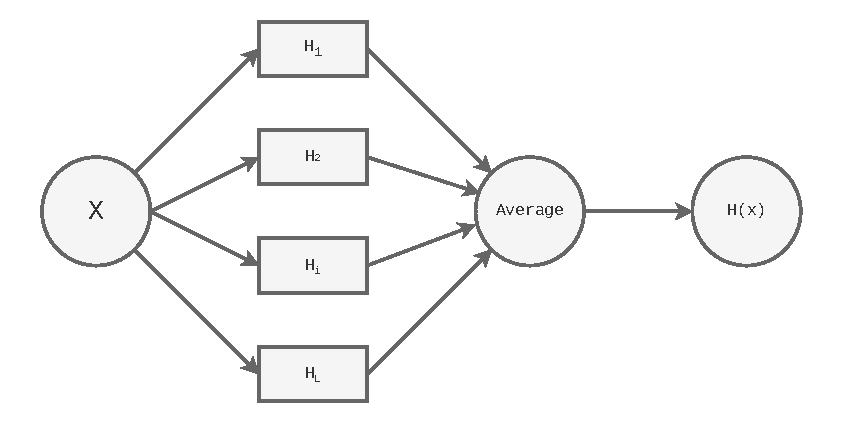
\includegraphics[width=0.8\textwidth]{images/el_averaging.pdf}
    \caption{Esempio di ensemble learning tramite averaging: esistono $L$ modelli $H_1, H_2, \ldots, H_L$ che fanno previsioni su un dato input $x$. La previsione finale $H(x)$ è la media delle previsioni dei modelli base.}
    \label{fig:el-averaging}
\end{figure}

Un primo metodo di fare ensemble learning è l'\textbf{averaging}, che consiste nel calcolare la media delle previsioni dei modelli base. Questo metodo è particolarmente utile per problemi di regressione, dove la previsione finale $H(x)$ è data da:
\[
H(x) = \frac{1}{L} \sum_{i=1}^{L} h_i(x)
\]

\subsection{Weighted Averaging}

\begin{figure}[htbp]
    \centering
    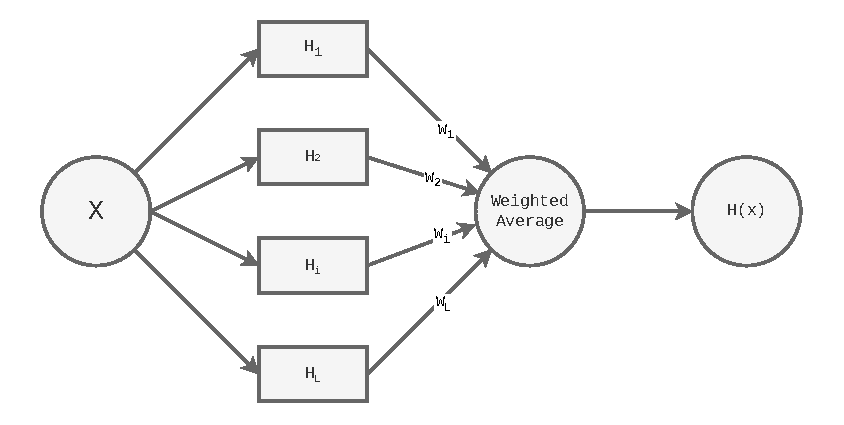
\includegraphics[width=0.8\textwidth]{images/el_weighted_averaging.pdf}
    \caption{Esempio di ensemble learning tramite weighted averaging: ogni modello $H_i$ ha un peso associato $w_i$ che riflette la sua affidabilità. La previsione finale $H(x)$ è una media pesata delle previsioni dei modelli base.}
    \label{fig:el-weighted-averaging}
\end{figure}

Un'estensione dell'averaging è il \textbf{weighted averaging}, dove ogni modello base ha un peso associato $w_i$ che riflette la sua affidabilità. L'idea è di dare più importanza ai modelli che performano meglio. La previsione finale è calcolata come:
\[
H(x) = \frac{\sum_{i=1}^{L} w_i h_i(x)}{\sum_{i=1}^{L} w_i}
\]

\subsection{Gating}

\begin{figure}[htbp]
    \centering
    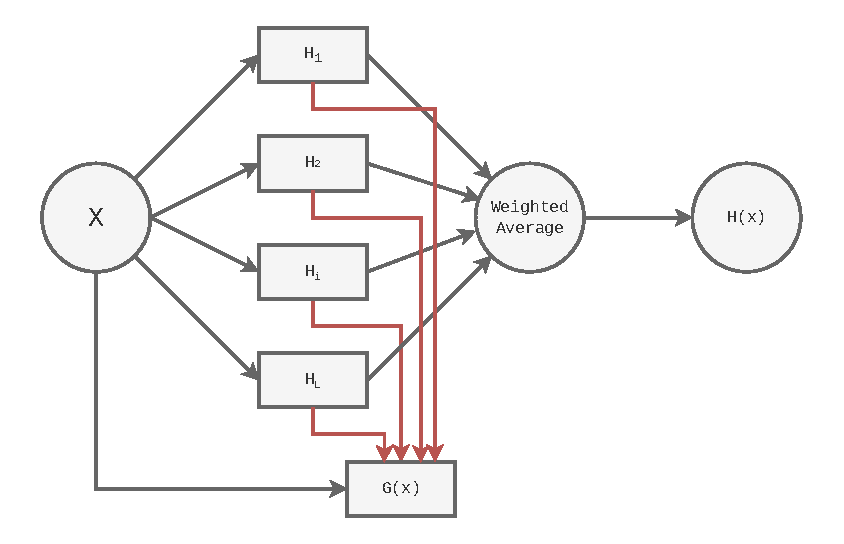
\includegraphics[width=0.8\textwidth]{images/el_gating.pdf}
    \caption{Esempio di ensemble learning tramite gating: un modello di gating $g(x)$ seleziona quale modello base utilizzare per fare la previsione finale $H(x)$.}
    \label{fig:el-gating}
\end{figure}

Un metodo più sofisticato di ensemble learning è il \textbf{gating}, in cui un modello di gating $g(x)$ decide quale modello base utilizzare per fare la previsione finale. Questo approccio è particolarmente utile quando i modelli base sono specializzati in diverse regioni dello spazio delle caratteristiche. La previsione finale è data da:
\[
H(x) = h_{g(x)}(x)
\]
dove $g(x)$ restituisce l'indice del modello base da utilizzare per l'input $x$.

\subsection{Stacking}


Un altro approccio è lo \textbf{stacking}, in cui le previsioni dei modelli base vengono utilizzate come input per un modello di livello superiore (detto \textit{meta-learner}) $C$ allenato su un \emph{validation set}. Questo è utile perché permette al meta-learner di apprendere come combinare le previsioni dei modelli base in modo ottimale. Si può formalizzare come:
\[
H(x) = C(h_1(x), h_2(x), \ldots, h_L(x))
\]

\begin{figure}[htbp]
    \centering
    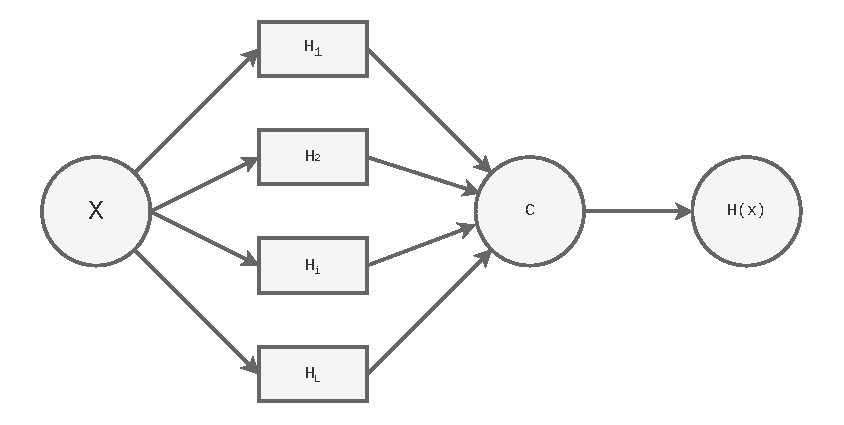
\includegraphics[width=0.8\textwidth]{images/el_stacking.pdf}
    \caption{Esempio di ensemble learning tramite stacking: le previsioni dei modelli base $H_1, H_2, \ldots, H_L$ vengono utilizzate come input per un modello di livello superiore (meta-learner) $C$ che produce la previsione finale $H(x)$.}
    \label{fig:el-stacking}
\end{figure}

\section{Tecniche di Manipolazione dei Dati}
Per migliorare la diversità tra i modelli base, l'ensemble learning spesso utilizza tecniche di manipolazione dei dati per creare diversi sottoinsiemi di dati di addestramento. Il vantaggio di questa diversità è che modelli diversi possono catturare differenti aspetti del problema, riducendo il rischio di overfitting e migliorando la generalizzazione.

\subsection{Boostrap replication}
Una tecnica comune è la \textbf{boostrap replication}, che consiste nel creare diversi sottoinsiemi di dati di addestramento campionando con ripetizione dal dataset originale. Ogni modello base viene addestrato su un sottoinsieme diverso, aumentando la diversità tra i modelli.

Dato un dataset $D$ con $n$ campioni, si creano $L$ sottoinsiemi $D_1, D_2, \ldots, D_L$ ciascuno ottenuto campionando $n$ volte con ripetizione da $D$. Ogni modello base $h_i$ viene quindi addestrato su $D_i$. Poiché il campionamento è con ripetizione, circa il 36.8\% dei campioni originali non verrà incluso in ciascun sottoinsieme, favorendo la diversità tra i modelli.

\subsection{Bagging}
Un'altra tecnica è il \textbf{bagging} (bootstrap aggregating), che combina la boostrap replication con l'averaging. In questo approccio, si creano diversi sottoinsiemi di dati di addestramento tramite boostrap replication, si addestrano modelli base su ciascun sottoinsieme e si combinano le loro previsioni tramite averaging o weighted averaging. Questo metodo è particolarmente efficace per ridurre la varianza dei modelli base, migliorando la stabilità e la performance complessiva dell'ensemble.

\subsection{Boosting}
Il \textbf{boosting} è una tecnica di ensemble learning che mira a creare un forte modello combinando molti modelli deboli in \textbf{sequenza}. A differenza del bagging, dove i modelli base sono indipendenti, nel boosting ogni modello successivo viene addestrato per correggere gli errori del modello precedente. Questo processo iterativo porta a un miglioramento continuo delle performance dell'ensemble.

\section{AdaBoost}
Adaboost (Adaptive Boosting) è uno degli algoritmi di boosting più popolari e ampiamente utilizzati. Costruisce un classificatore forte come combinazione pesata di $T$ classificatori deboli (weak hypotheses) $h_t$, enfatizzando iterativamente gli esempi misclassificati tramite pesi d'istanza $w_{t,i}$.

\paragraph{Input e notazione.}
Sia il training set $(X,y)=\{(x_i,y_i)\}_{i=1}^n$ e sia $T$ il numero di iterazioni.
I pesi al passo $t$ sono $w_t=(w_{t,1},\dots,w_{t,n})$ e $h_t$ è il modello allenato al passo $t$.

\subsection{Algoritmo}
Si può descrivere cosa fanno i vari passi dell'algoritmo in questo modo:

\begin{enumerate}
\item \textbf{Initialize a vector of $n$ uniform weights}\\
Inizializza una distribuzione uniforme sugli esempi:
\[
w_1=\Big[\tfrac{1}{n},\ldots,\tfrac{1}{n}\Big].
\]
Interpretazione: all'inizio tutti gli esempi contano uguale.

\item \textbf{for $t=1,\ldots,T$}\\
Ciclo di boosting: ad ogni iterazione si costruisce un nuovo weak learner che si concentra sugli esempi più ``difficili'' (quelli con peso alto).

\item \textbf{Train model $h_t$ on $X,y$ with instance weights $w_t$}\\
Allena $h_t$ usando i pesi $w_t$: gli esempi con $w_{t,i}$ maggiore influenzano di più il training (equivalente a ``replicare'' più volte quegli esempi). 

\item \textbf{Compute the weighted training error rate of $h_t$:}\\
\[
\varepsilon_t=\sum_{i: y_i\neq h_t(x_i)} w_{t,i}.
\]
Interpretazione: è la probabilità (secondo la distribuzione $w_t$) che $h_t$ sbagli; non è un errore ``non pesato'', ma un errore misurato rispetto ai pesi correnti.

\item \textbf{Choose $\alpha_t=\tfrac12 \ln\!\Big(\frac{1-\varepsilon_t}{\varepsilon_t}\Big)$}\\
\[
\alpha_t=\frac{1}{2}\ln\Big(\frac{1-\varepsilon_t}{\varepsilon_t}\Big).
\]
Interpretazione: $\alpha_t$ è il peso del weak learner nell'ensemble finale.
Se $\varepsilon_t$ è piccolo (modello buono), $\alpha_t$ è grande; se $\varepsilon_t\approx 0.5$, $\alpha_t\approx 0$. 

\item \textbf{Update all instance weights:}\\
\[
w_{t+1,i}=w_{t,i}\exp\big(-\alpha_t\, y_i\, h_t(x_i)\big)\qquad \forall i=1,\ldots,n.
\]
Cosa fa \emph{di preciso}:
\begin{itemize}
\item se $y_i=h_t(x_i)$ (predizione corretta), allora $y_i h_t(x_i)=+1$ e
$w_{t+1,i}=w_{t,i}e^{-\alpha_t}$: il peso \emph{diminuisce}.
\item se $y_i\neq h_t(x_i)$ (predizione errata), allora $y_i h_t(x_i)=-1$ e
$w_{t+1,i}=w_{t,i}e^{+\alpha_t}$: il peso \emph{aumenta}.
\end{itemize}
Quindi i punti sbagliati vengono enfatizzati e i punti corretti ``svalutati''.

\item \textbf{Normalize $w_{t+1}$ to be a distribution:}\\
\[
w_{t+1,i}=\frac{w_{t+1,i}}{\sum_{j=1}^{n} w_{t+1,j}}\qquad \forall i=1,\ldots,n.
\]
Interpretazione: si riporta la somma dei pesi a $1$ così che $w_{t+1}$ resti una distribuzione di probabilità sugli esempi.

\item \textbf{end for}\\
Dopo $T$ iterazioni si hanno $T$ weak learners e i rispettivi pesi $\alpha_t$.
\item \textbf{Return the hypothesis}\\
\[
H(x)=\operatorname{sign}\left(\sum_{t=1}^{T}\alpha_t h_t(x)\right).
\]
Interpretazione: è un voto pesato (somma pesata delle predizioni); la $\operatorname{sign}(\cdot)$ restituisce la classe finale.
\end{enumerate}

\begin{algorithm}[htbp]
\caption{AdaBoost}
\begin{algorithmic}[1]
\Require Training set $\{(x_i,y_i)\}_{i=1}^n$ with $y_i\in\{-1,+1\}$, number of rounds $T$
\Ensure Final hypothesis $H$

\State Initialize $w_{1,i} \gets \frac{1}{n}$ for $i=1,\ldots,n$
\For{$t=1,\ldots,T$}
    \State Train weak learner $h_t$ on $\{(x_i,y_i)\}_{i=1}^n$ using weights $w_t$
    \State $\varepsilon_t \gets \sum_{i: y_i \neq h_t(x_i)} w_{t,i}$
    \State $\alpha_t \gets \frac{1}{2}\ln\left(\frac{1-\varepsilon_t}{\varepsilon_t}\right)$
    \For{$i=1,\ldots,n$}
        \State $w_{t+1,i} \gets w_{t,i}\exp\!\big(-\alpha_t\,y_i\,h_t(x_i)\big)$
    \EndFor
    \State Normalize: $w_{t+1,i} \gets \frac{w_{t+1,i}}{\sum_{j=1}^n w_{t+1,j}}$ for $i=1,\ldots,n$
\EndFor
\State \Return $H(x) = \operatorname{sign}\left(\sum_{t=1}^T \alpha_t h_t(x)\right)$
\end{algorithmic}
\end{algorithm}

\subsection{Caso studio: Two moons dataset}
Il dataset \emph{two moons} è un dataset sintetico molto utilizzato per testare algoritmi di classificazione, in particolare quelli che devono catturare relazioni non lineari tra le caratteristiche. Il dataset è composto da due classi a forma di mezzaluna che si intrecciano, rendendo difficile la separazione lineare.

Per il funzionamento che ha AdaBoost, questo dataset è particolarmente interessante perché mostra come l'algoritmo possa costruire un ensemble di weak learners (ad esempio, decision stumps) che, combinati, riescono a catturare la complessità del dataset e a separare efficacemente le due classi (nonostante ogni weak learner sia lineare e non sia in grado di separare le classi da solo).

\paragraph{Decision boundary.}
Questo avviene perché AdaBoost, iterativamente, si concentra sugli esempi più difficili (quelli vicini alla frontiera di decisione) e costruisce weak learners che cercano di correggere gli errori dei modelli precedenti. 

Ricordando che il Decision Boundary di un classificatore è la frontiera che separa le diverse classi nello spazio delle caratteristiche, in AdaBoost questa frontiera evolve man mano che si aggiungono nuovi weak learners all'ensemble. All'inizio, con pochi weak learners, il decision boundary può essere semplice e lineare. Man mano che si aggiungono più weak learners, il decision boundary diventa più complesso e capace di catturare le caratteristiche non lineari dei dati, come nel caso del dataset two moons.

Nella Figura \ref{fig:adaboost-boundaries} si mostra come il decision boundary di AdaBoost cambia dopo diverse iterazioni (1, 12, 25 e 50). Si può notare che inizialmente il boundary è semplice e lineare, ma con l'aggiunta di più weak learners diventa sempre più complesso, riuscendo a catturare la forma non lineare del dataset.

\begin{figure}[H]
    \centering
    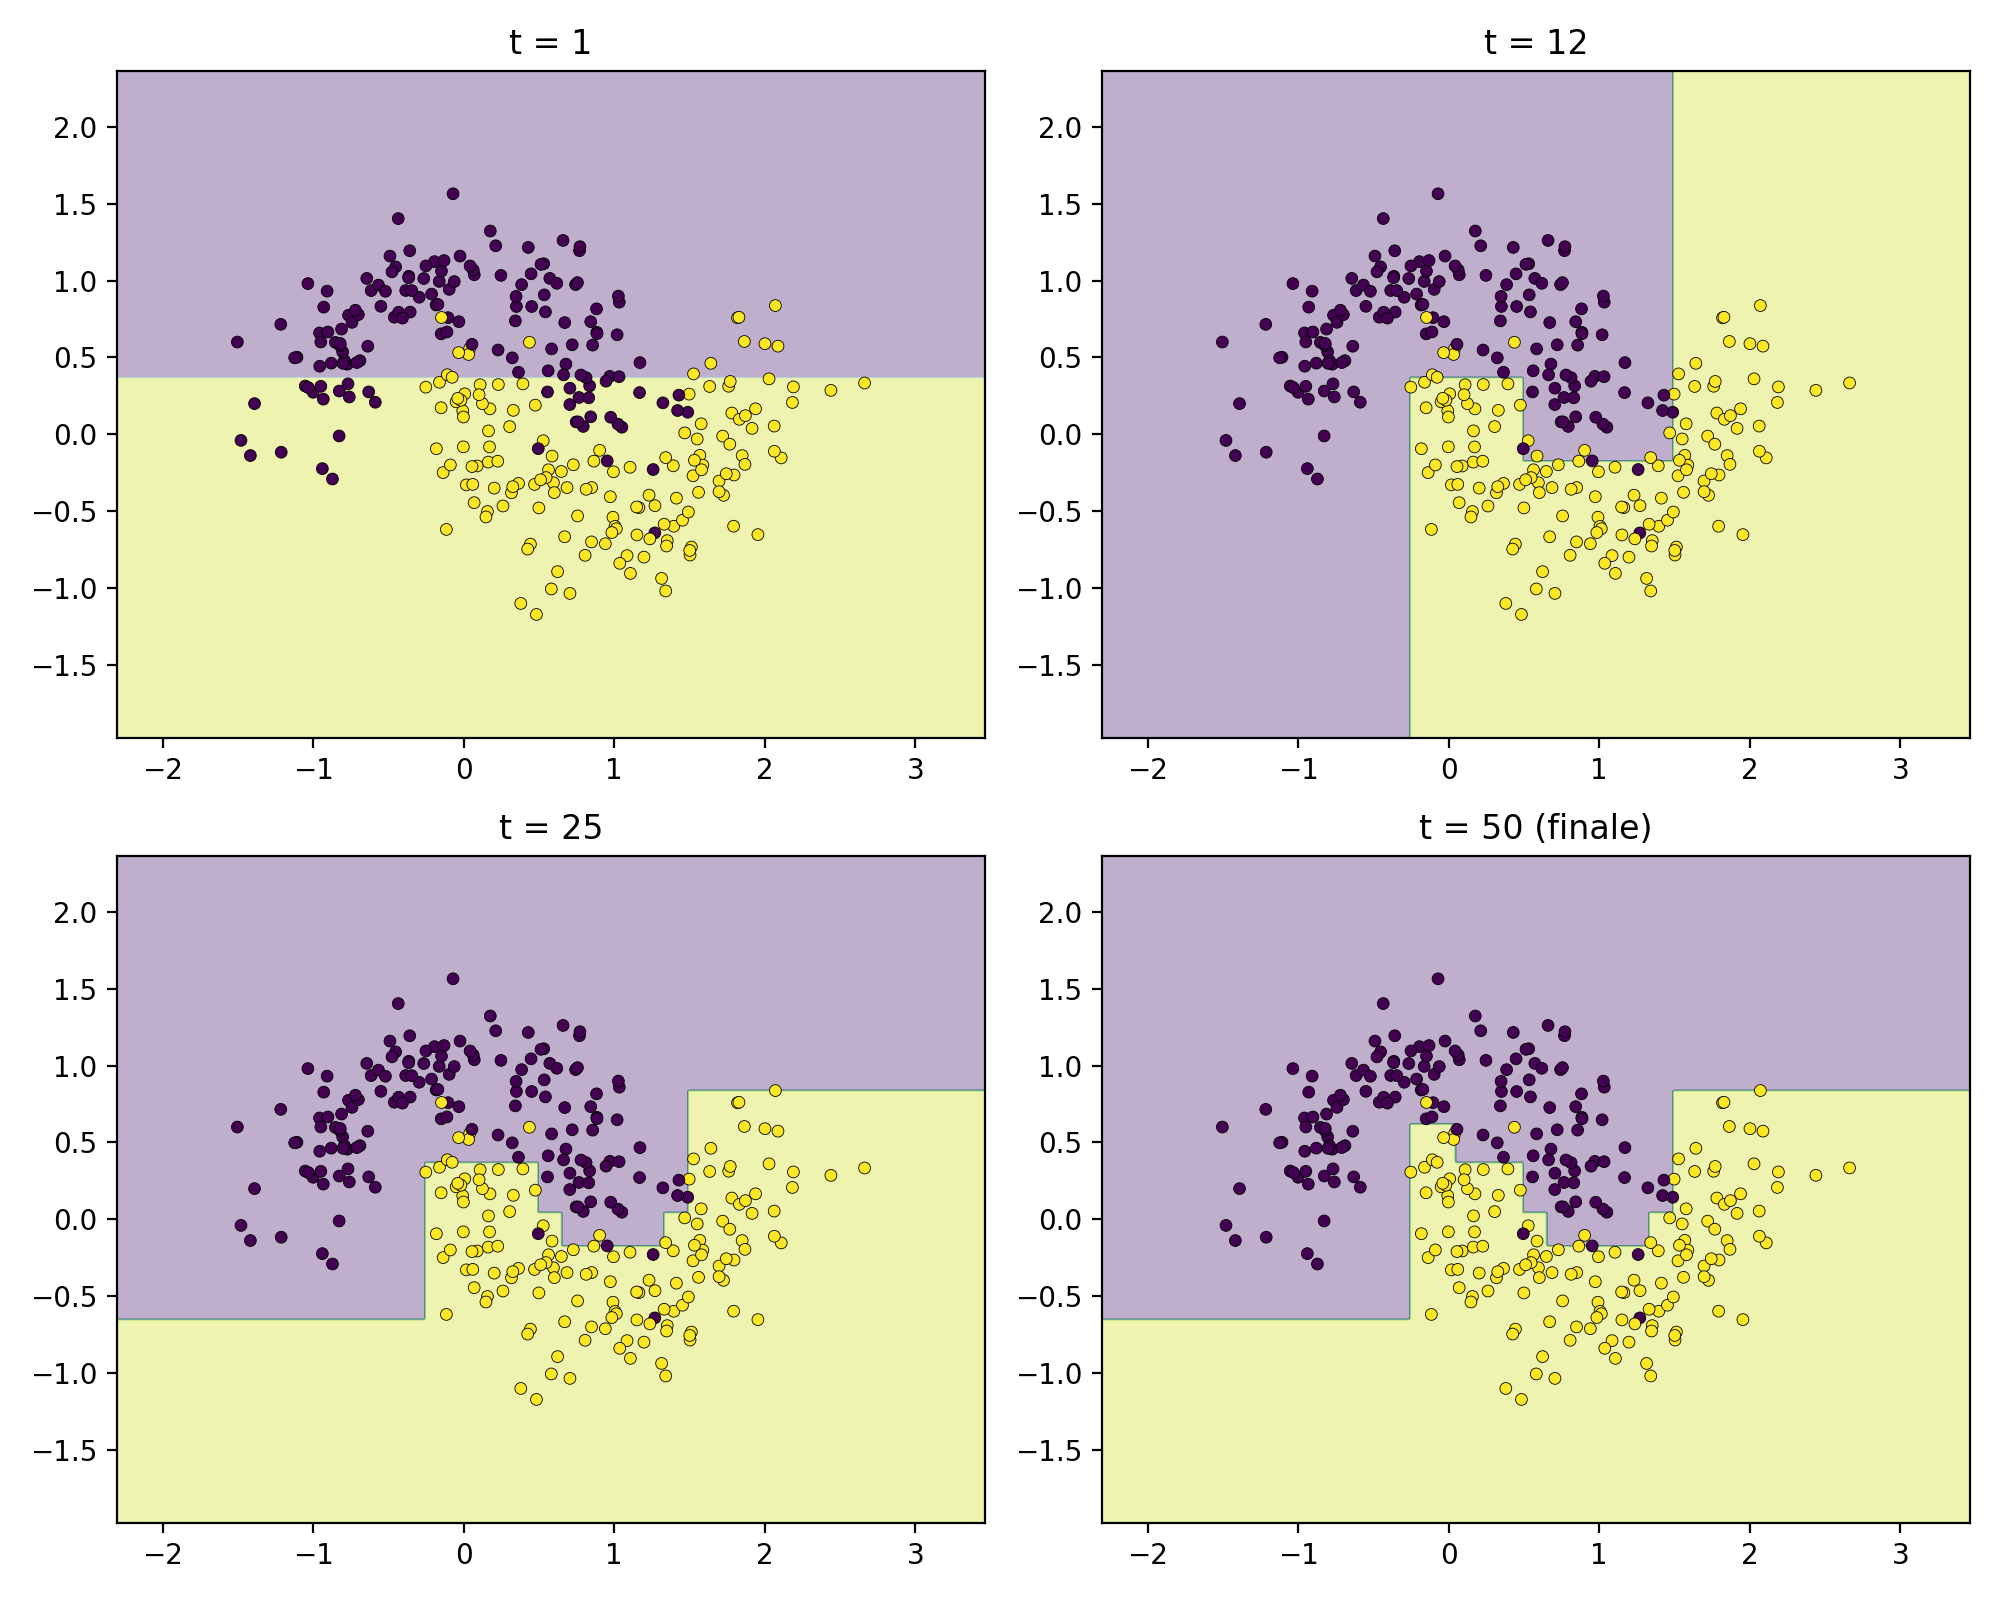
\includegraphics[width=1\textwidth]{images/adaboost_boundaries.png}
    \caption{Evoluzione del decision boundary di AdaBoost al crescere del numero di iterazioni. 
    In alto a sinistra è mostrato il boundary dopo la prima iterazione ($t=1$), in alto a destra dopo $t=12$, 
    in basso a sinistra dopo $t=25$ e in basso a destra il decision boundary finale ($t=50$). 
    Si osserva come la combinazione sequenziale di weak learners permetta di approssimare progressivamente 
    una frontiera di decisione non lineare, concentrandosi sulle regioni di maggiore difficoltà.}
   \label{fig:adaboost-boundaries}
\end{figure}

\section*{Riferimenti}
I riferimenti principali per questo capitolo sono:
\begin{itemize}
    \item Materiale visto a lezione.
    \item Materiale sul boosting e AdaBoost dal capitolo 17 del libro \citetitle{Alpaydin2014} \cite{Alpaydin2014}.
\end{itemize}